\documentclass[10pt,svgnames]{beamer}
\usepackage[portuguese]{babel} 
\usepackage[utf8]{inputenc}
\usepackage{amssymb,amsmath}
\usepackage{listings}
\usepackage{palatino}
\usepackage{beamerthemesplit}

\usetheme{Rochester}
\usecolortheme{dolphin}
 
\title{Tabelas Hash}
\author[DAD-II - Lucas H. Negri]{Lucas Hermann Negri}
\institute{Departamento de Ciência da Computação (DCC) \\ Centro de Ciências Tecnológicas (CCT)  \\ Universidade do Estado de Santa Catarina (UDESC)} 

\date{11 de Abril de 2013}

\def\hilite<#1>{
\temporal<#1>{\color{black}}{\color{blue}}
{\color{black}}}

\newenvironment{mitemize}{\begin{itemize} \itemsep=1cm}{\end{itemize}}

\begin{document} 

\frame{ \titlepage }

\frame{ \frametitle{Tópicos} \tableofcontents }

\section{Introdução}

\frame{
    \frametitle{Definição}
    
    Uma tabela hash é uma estrutura utilizada no mapeamento de chaves para seus respectivos valores.
    Por exemplo, um dicionário é uma estrutura que mapeia (relaciona) palavras aos seus significados.
}

\frame{
    \frametitle{Operações Básicas}
    
    Uma tabela hash atua como uma estrutura de dicionário ou vetor associativo, e suporta as seguintes operações básicas~\cite{cormen}:
    
    \begin{itemize}
    \item Inserção
    \item Busca
    \item Remoção
    \end{itemize}
    
    Sob hipóteses razoáveis (veremos adiante), todas as três operações podem ser implementadas com complexidade
    computacional próxima de $O(1)$.
}

\subsection{Tabelas de endereço direto}

\frame{
    \frametitle{Tabelas de endereço direto}
    
    \begin{mitemize}
    \item Utilizável quando o universo de chaves é suficientemente pequeno e representado por inteiros
    \item Para uma caso simplificado sem colisões de chaves, equivale ao uso de vetores, onde cada posição do
    vetor corresponde ao espaço na tabela para a entrada de chave igual à posição
    \end{mitemize}
}

\frame{
    \frametitle{Exemplo de tabela de endereço direto}
    
    \begin{figure}[tbp]
    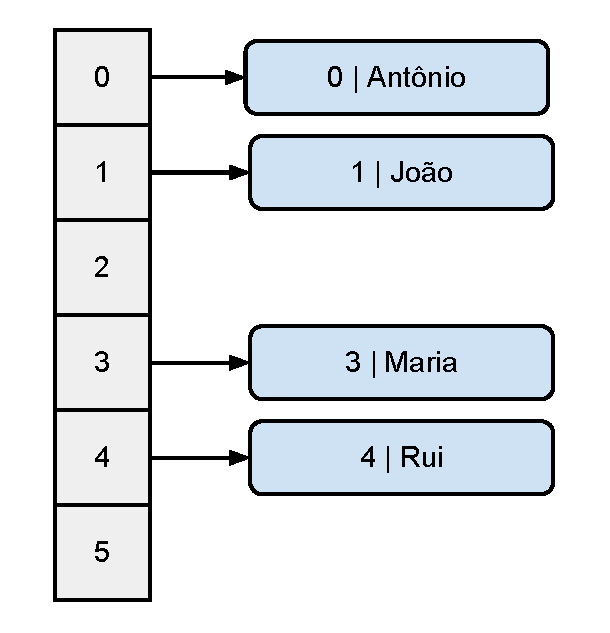
\includegraphics[keepaspectratio=true,width=2.25in]{res/endereco_direto}
    \centering
    \caption{Tabela de endereço direto}
    \end{figure}
}

\begin{frame}[fragile]
\frametitle{Tabela de endereço direto - Inserção}
\begin{verbatim}
INSERÇÃO(TABELA, DADO) {
    TABELA[ DADO->CHAVE ] = DADO
}
\end{verbatim}
\end{frame}

\begin{frame}[fragile]
\frametitle{Tabela de endereço direto - Busca}
\begin{verbatim}
BUSCA(TABELA, CHAVE) {
    return TABELA[ CHAVE ]
}
\end{verbatim}
\end{frame}

\begin{frame}[fragile]
\frametitle{Tabela de endereço direto - Remoção}
\begin{verbatim}
REMOÇÃO(TABELA, CHAVE) {
    TABELA[ CHAVE ] = NULO
}
\end{verbatim}
\end{frame}

\subsection{Tabelas hash}

\frame{
    \frametitle{Tabelas hash}
    
    No endereçamento direto teremos problemas nos seguintes casos:
    
    \begin{itemize}
    \item O universo (a faixa) de chaves é muito grande
    \item Os dados que deverão ser armazenados não possuem chaves numéricas
    \end{itemize}
    
    A solução está no uso de uma função de hash que faça o mapeamento de uma chave para um endereço
    válido de uma tabela.
}

\frame{
    \frametitle{Exemplo de tabela hash}
    
    \begin{figure}[tbp]
    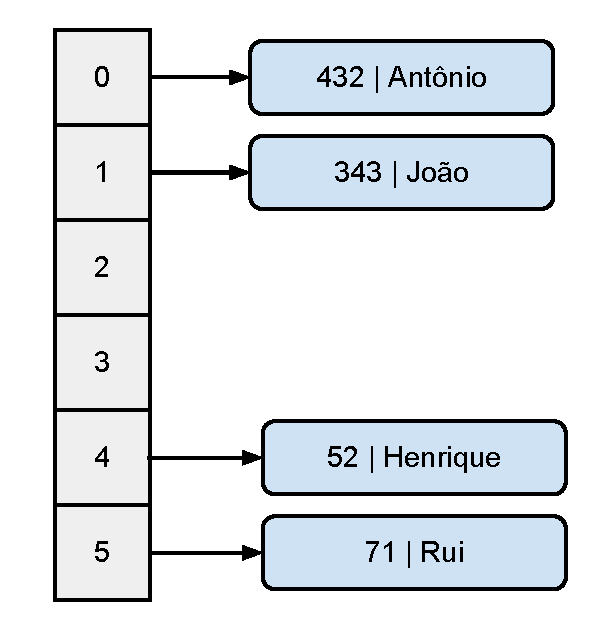
\includegraphics[keepaspectratio=true,width=2.25in]{res/tabela_hash_1}
    \centering
    \caption{Tabela hash}
    \end{figure}
}

\begin{frame}[fragile]
\frametitle{Tabela hash - Inserção}
\begin{verbatim}
INSERÇÃO(TABELA, DADO) {
    ENDEREÇO = HASH( DADO->CHAVE )
    TABELA[ ENDEREÇO ] = DADO
}
\end{verbatim}
\end{frame}

\begin{frame}[fragile]
\frametitle{Tabela hash - Busca}
\begin{verbatim}
BUSCA(TABELA, CHAVE) {
    ENDEREÇO = HASH( CHAVE )
    return TABELA[ ENDEREÇO ]
}
\end{verbatim}
\end{frame}

\begin{frame}[fragile]
\frametitle{Tabela hash - Remoção}
\begin{verbatim}
REMOÇÃO(TABELA, CHAVE) {
    ENDEREÇO = HASH( CHAVE )
    TABELA[ ENDEREÇO ] = NULO
}
\end{verbatim}
\end{frame}

\section{Funções de Hash}

\frame{
    \frametitle{Funções de hash}
    
    \textbf{Necessidade: mapeamento da chave para um endereço.}
    \\[2em]
    Muitas vezes os dados que serão armazenados não possuem chaves numéricas (ou sua faixa é muito grande) e é necessário
    mapear um dado de outro tipo (como uma cadeia de caracteres) para um endereço.
}

\frame{
    \frametitle{Funções de hash}
    
    \textbf{Necessidade: boa distribuição de endereços.}
    \\[2em]
    Na maioria das situações práticas, salvo aquelas nas quais os dados são conhecidos com antecedência e é possível
    realizar um hashing perfeito, uma função de hash irá retornar o mesmo endereço para diferentes dados em algum momento, gerando uma colisão.
}

\frame{
    \frametitle{Construção de uma boa função de hash}
    Logo, a função de hash utilizada deve:
    
    \begin{itemize}
    \item Mapear a chave para um endereço válido
    \item Ter uma boa distribuição de forma a minimizar as colisões
    \item Ser eficiente
    \end{itemize}
}

\subsection{Funções para chaves inteiras}

\frame{
    \frametitle{Hash de chaves inteiras}
    
    Exemplos de funções de hash para chaves inteiras~\cite{cormen}:
    
    \begin{itemize}
    \item Método da divisão
    \item Método da multiplicação
    \end{itemize}
    
    Aqui definimos $M$ como o número de endereços na tabela.
}

\begin{frame}[fragile]
\frametitle{Funções de hash - método da divisão}
\begin{verbatim}
HASH(CHAVE, M) {
    return CHAVE mod M
}
\end{verbatim}
\end{frame}

\frame{
    \frametitle{Método da divisão}
    
    Características:
    
    \begin{itemize}
    \item Método simples e rápido de ser computado
    \item Pode ter uma distribuição ruim dependendo do valor de $M$\footnote{ex.: $M$ não deve ser uma potência de $2$}
    \end{itemize}
}

\begin{frame}[fragile]
\frametitle{Funções de hash - método da multiplicação}
\begin{verbatim}
HASH(CHAVE, M) {
    AUX = M * ( (CHAVE * TAXA) mod 1)
    return floor( AUX )
}
\end{verbatim}
\end{frame}

\frame{
    \frametitle{Método da multiplicação}
    
    Características:
    
    \begin{itemize}
    \item A distribuição não é dependente do valor de $M$
    \item Funciona com qualquer valor de TAXA, mas a literatura sugere um valor próximo a $$(\sqrt{5}-1)/2 = 0,6180339887...$$
    \end{itemize}
}

\subsection{Funções para cadeias de caracteres}

\frame{
    \frametitle{Para cadeias de caracteres}
    
    \begin{itemize}
    \item Somatório (ruim)
    \item djb2
    \end{itemize}
}

\begin{frame}[fragile]
\frametitle{Funções de hash - somatório}
\begin{verbatim}
HASH(CHAVE, M) {
    AUX = 0
    
    PARA CADA CARACTERE C EM CHAVE {
        AUX = AUX + C
    }
    
    return AUX mod M
}
\end{verbatim}
\end{frame}

\begin{frame}[fragile]
\frametitle{Funções de hash - djb2}
\begin{verbatim}
HASH(CHAVE, M) {
    AUX = 5381
    
    PARA CADA CARACTERE C EM CHAVE {
        AUX = AUX * 33 + C
    }
    
    return AUX mod M
}
\end{verbatim}
\end{frame}

\section{Resolução de Colisões}

\frame{
    \frametitle{Resolução de Colisões}
    
    \begin{mitemize}
    \item Salvo situações especiais, chaves diferentes serão mapeadas para a mesma posição,
    causando assim uma \emph{colisão}
    \item Boas funções de \emph{hash} diminuem o número de colisões, mas em uma situação normal elas
    irão ocorrer, logo a tabela deve tratar colisões
    \item Dois métodos comuns: por encadeamento e por endereçamento aberto
    \end{mitemize}
}

\subsection{Encadeamento}

\frame{
    \frametitle{Resolução de Colisões por Encadeamento}
    
    \begin{figure}[tbp]
    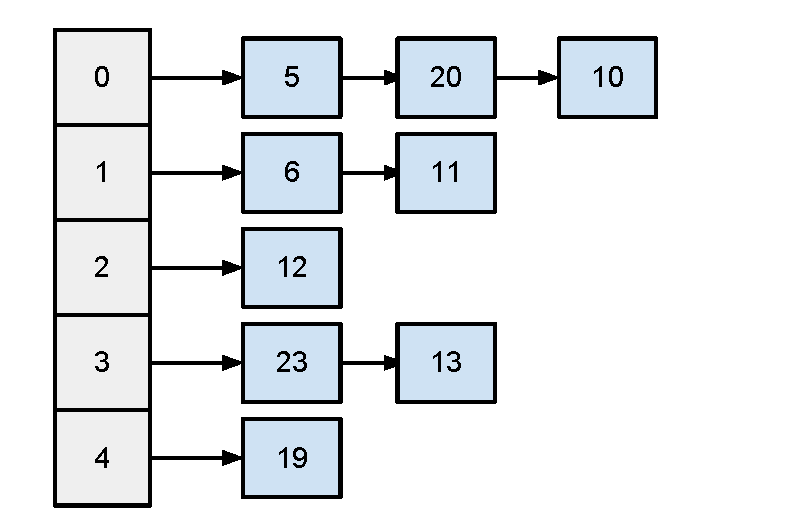
\includegraphics[keepaspectratio=true,width=3.5in]{res/encadeamento}
    \centering
    \caption{Resolução de colisões por encadeamento (end = chave mod 5) }
    \end{figure}
}


\begin{frame}[fragile]
\frametitle{Tabela hash (encadeamento) - Inserção}
\begin{verbatim}
INSERÇÃO(TABELA, DADO) {
    ENDEREÇO = HASH( DADO->CHAVE )
    INSERE_LISTA( TABELA[ ENDEREÇO ], DADO )
}
\end{verbatim}
\end{frame}

\begin{frame}[fragile]
\frametitle{Tabela hash (encadeamento) - Busca}
\begin{verbatim}
BUSCA(TABELA, CHAVE) {
    ENDEREÇO = HASH( CHAVE )
    return BUSCA_LISTA( TABELA[ ENDEREÇO ], CHAVE )
}
\end{verbatim}
\end{frame}

\begin{frame}[fragile]
\frametitle{Tabela hash (encadeamento) - Remoção}
\begin{verbatim}
REMOÇÃO(TABELA, CHAVE) {
    ENDEREÇO = HASH( CHAVE )
    REMOVE_LISTA( TABELA[ ENDEREÇO ], CHAVE )
}
\end{verbatim}
\end{frame}

\subsection{Endereçamento aberto}

\frame{
    \frametitle{Endereçamento aberto}
    
    \begin{itemize}
    \item Todos os elementos são armazenados na própria tabela
    \item Quando há uma colisão, escolhe-se uma nova posição para o novo dado
    \item A tabela pode ficar cheia, necessitando de redimensionamento
    \item As operações utilizam o processo de sondagem para encontrar a posição de um elemento
    \end{itemize}
}

\frame{
    \frametitle{Endereçamento aberto}
    
    \begin{figure}[tbp]
    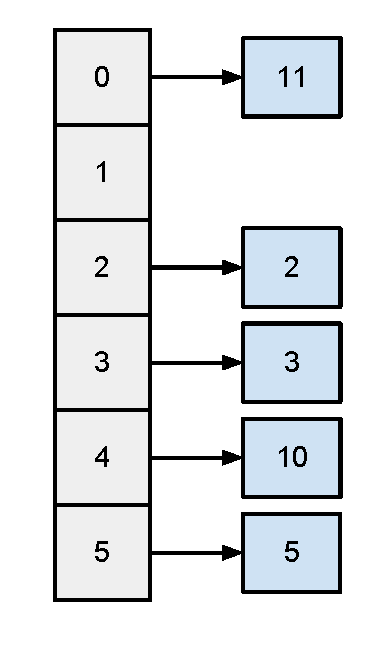
\includegraphics[keepaspectratio=true,width=1.25in]{res/aberto}
    \centering
    \caption{Endereçamento aberto, onde hash(chave) = chave \% M }
    \end{figure}
}

\begin{frame}[fragile]
\frametitle{Tabela hash (endereçamento aberto) - Inserção}
\begin{verbatim}
INSERÇÃO(TABELA, DADO) {
    I = 0
    
    FAÇA
        ENDEREÇO = HASH'( DADO->CHAVE, I )
        
        SE TABELA[ ENDEREÇO ] ESTÁ VAZIA
            TABELA[ ENDEREÇO ] = DADO
            return
        SENÃO
            I = I + 1
    ATÉ QUE I = M
    
    ERRO("TABELA CHEIA")
}
\end{verbatim}
\end{frame}

\begin{frame}[fragile]
\frametitle{Tabela hash (endereçamento aberto) - Busca}
\begin{verbatim}
BUSCA(TABELA, CHAVE) {
    I = 0
    
    FAÇA
        ENDEREÇO = HASH'( CHAVE, I )
        
        SE TABELA[ ENDEREÇO ] = CHAVE
            return TABELA[ ENDEREÇO ]
        SENÃO
            I = I + 1
    ATÉ QUE TABELA[ENDEREÇO] = VAZIO OU I = M
    
    return NULO
}
\end{verbatim}
\end{frame}

\begin{frame}[fragile]
\frametitle{Tabela hash (endereçamento aberto) - Remoção}
\begin{verbatim}
REMOÇÃO(TABELA, CHAVE) {
    I = 0
    
    FAÇA
        ENDEREÇO = HASH'( CHAVE, I )
        
        SE TABELA[ ENDEREÇO ] = CHAVE
            TABELA[ ENDEREÇO ] = REMOVIDO
            return TRUE
        SENÃO
            I = I + 1
    ATÉ QUE TABELA[ENDEREÇO] = VAZIO OU I = M
    
    return FALSE
}
\end{verbatim}
\end{frame}

\frame{
    \frametitle{Sondagem linear}
    
    \begin{equation}
    hash'(chave, i) = (hash(chave) + i) \% M
    \end{equation}
}

\frame{
    \frametitle{Sondagem quadrática}
    
    \begin{equation}
    hash'(chave, i) = (hash(chave) + c_{1} i + c_{2} i^{2}) \% M
    \end{equation}
}

\bibliographystyle{unsrt}
\renewcommand\refname{Referências}

\frame{
    \frametitle{Referências}
    \bibliography{pres}
}

\end{document}
